\chapter{Electronics} % (fold)
\label{chap:electronics}

This chapter describes the implementation of a solution that enables detection of point of impact for a ping pong ball using an FPGA and piezo electric elements.

This section describes the construction of a number of sensor circuits using piezo electric elements to measure the time of arrival of bending waves.
There is a circuit like the one on figure \ref{fig:print} for each sensor. It is chosen to make one print for each circuit in order to keep the wires conducting the analog sensor values as small as possible. 
\begin{figure}[htb]
	\centering
	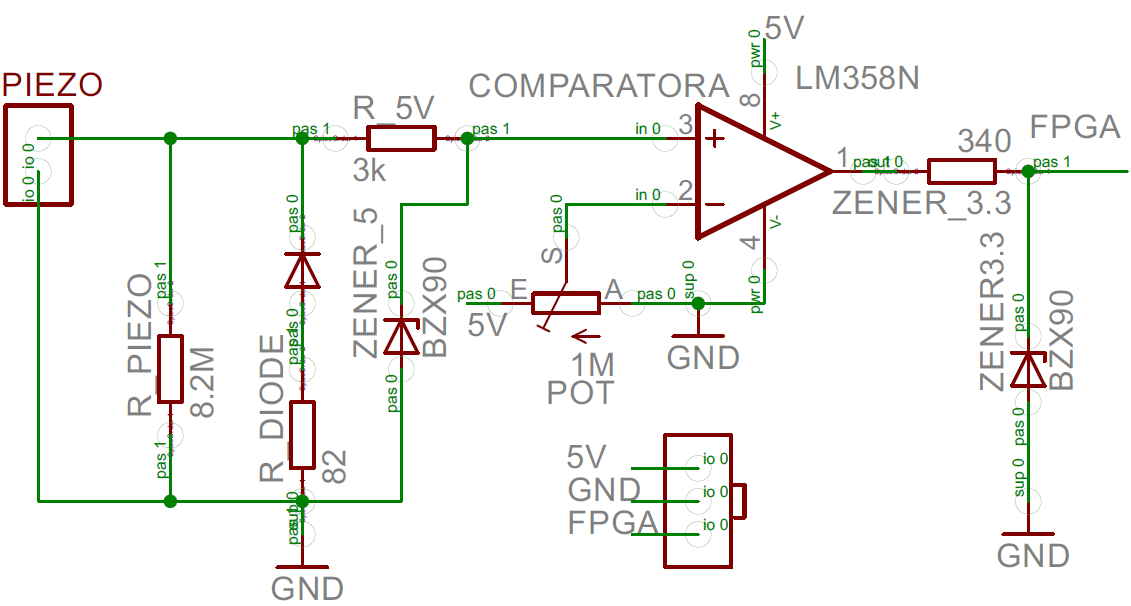
\includegraphics[width=1.\textwidth]{figures/Print}
	\caption{Schematics of circuit for digitalizing the output from a piezo electric elements.}
	\label{fig:print}
\end{figure}
The very small current that the piezo electric element generates are amplified with a resistor on $8.5M\si{\ohm}$. This value is chosen since test showed that it was possible to detect ball bounce from as low a hight as $30\si{\centi\meter}$.
Diodes are used to account for the large positive and negative voltage spikes that the sensor in combination with the large resistor can output in case of a powerful input to the sensor. 
Since the negative voltage are not use it is removed up to $0.7V$ with a diode which conducts current for ground when the voltage from the piezo becomes less then $0.7V$.
The resistor is calculated according to equation \ref{eq:distDifference}.
\begin{equation}
 20 - 0.7 V = R_{diode} \cdot 300mA \Leftrightarrow R_{diode} = 64.3\si{\ohm}
 \label{diodeResistor}
\end{equation}
%Since this resistance was not in stock a resistor of $82 {\si{\ohm}$ is chosen.
Where the $20V$ is taken as a guess on the absolute maximum based on the fact that tests has not shown voltages above $15V$ when throwing the ball against the plate. Hence the system are robust against misuse.
Since the op-amp can not compare values that are larger than the supply of $5V$, the positive voltage is limited to $5.1V$ with a zener diode \cite{zener}. The resistor $R_5V$ is calculated by assuming infinite input resistance in the op amp according to equation 
\begin{equation}
%20 - 5 V = R_{5V} \cdot 5mA \Leftrightarrow R_{diode} = 3{k\si{\ohm}
\label{eq:zener5VResistor}
\end{equation}
A zener diode \cite{zener} is used to convert the $5V$ on the data output from the operational amplifier to $3.3V$, which is appropriate voltage for the FPGA. The solution with a zener diode is chosen over a another using a voltage divider since the voltage is kept at $3.3V$ for all op-amp of the type LM358 even in case of changes in production. According to the datasheet for LM358 the saturated output voltages varies from the supply voltages down to $1.5V$ below \cite{lm358}.
The resistor placed on the output of the operational amplifier is calculated using the current used for testing conditions in the datasheet for the diode, as can be seen in equation \ref{eq:zener} \cite{zener}.
\begin{equation}
5-3.3V = R_{z} I_{test} \Leftrightarrow R_{z} = 1.7V/5mA = 340\si{\ohm}
\label{eq:zener}
\end{equation}
% 
A potentiometer is connected to the inverting pin of the Op-amp in order to ease the tuning process. It's value is set to $1\si{\mega\ohm}$ to minimize the power consumption.

% chapter electronics (end)